\documentclass[conference]{IEEEtran}
\IEEEoverridecommandlockouts
% The following packages are commonly used in IEEE papers
\usepackage{cite}
\usepackage{amsmath,amssymb,amsfonts}
\usepackage{algorithmic}
\usepackage{graphicx}
\usepackage{textcomp}
\usepackage{xcolor}
\usepackage{tikz}
\usetikzlibrary{shapes.geometric, arrows, positioning}
\usepackage{caption}
\usepackage{subcaption}
\usepackage{float}
\usepackage{hyperref}
\usepackage{href-ul} % For underline 



\definecolor{linkscolors}{RGB}{120, 150, 220} % even softer muted blue-gray

\hypersetup{
  colorlinks=true,           % Enable colored links
  linkcolor=linkscolors,            % Color for internal links
  urlcolor=linkscolors,              % Color for external links
  citecolor=linkscolors,           % Color for citations
}


\title{CIFAR-100}
\author{\IEEEauthorblockN{Kevin Lopez}
\IEEEauthorblockA{
\textit{California State University Long Beach}\\
Long Beach, Ca \\
Kevin.LopezChavez01@student.csulb.edu}}
\date{\today}
% \textit{California State University Long Beach}\\
% email@domain.edu}}

\begin{document}

\maketitle

\section{Introduction} \label{sec: intro}
% This report details the activation functions, optimizers, hyper-parameters, and architectures used in the three best Convolutional Neural Network (CNN) models developed for the CIFAR-100 dataset. It includes their test accuracies, benchmarking results, the total number of parameters for each model, and visual diagrams of their architectures.
This report details the development and evaluation of three Convolutional Neural Network (CNN) models trained purely on the CIFAR-100 dataset.  It covers the experimental setup(in Section~\ref{sec: experimental setup}), multiple model evaluations (in Section~\ref{sec: models evaluation}), the model selection (in Section~\ref{sec: best model architectures}), the full retraining process (in Section~\ref{sec: full retrain}), and a comparison with top models in \href{https://paperswithcode.com/sota/image-classification-on-cifar-100 }{papers with code}.

% The models compare to the best models posted in \href{https://paperswithcode.com/sota/image-classification-on-cifar-100 }{papers with code} benchmarks. 
% Achieving high accuracy in CIFAR100 with models trained purely in that dataset is a challenging task because of the high number of classes (100), and the number of images per class is limited to 500. 
% TODO: Write me a sentence 


\section{Experimental Setup} \label{sec: experimental setup}
\subsection{Data Splitting}
The CIFAR-100 dataset is made up of 50,000 training images and 10,000 test images.
The training dataset was further divided into:
\begin{itemize}
    \item \textbf{Validation Set}: $\frac{1}{5}$ of entire training set =  10,000 images
    \item \textbf{Sub Train}: $Entire\_training\_set - \frac{1}{5} \times Entire\_training\_set$  = 40,000 images
\end{itemize}
This split was done using PyTorch's \texttt{random\_split} function.

\subsection{Data Transformation}
To make the models generalize better and reduce overfitting, I used data transformation and applied them to the entire training data. Transformations are the following:
\begin{itemize}
    \item Random Horizontal Flip
    \item Random Crop with padding
    \item Color Jittering (brightness, contrast, saturation, hue)
    \item Random Rotation
\end{itemize}
These transformations allowed me to achieve a 10 percent improvement compared to doing it without.
The same test was performed without data transformations and got 50 \% percent accuracy for all three models. While I have not attached the .ipynb file, it is available upon request.

\section{Model Evaluation with Ray Tune} \label{sec: models evaluation}
To start, I developed \textbf{8 different CNN architectures}.
Each architecture was trained using Ray Tune for hyper-parameter optimization and model selection.
Ray Tune was configured to run \textbf{16 models in parallel} using asynchronous hyperband scheduling, keeping the top 50\% of the models based on validation performance during training.
In total, \textbf{60 models} were evaluated using ray tune and were run up to a maximum of 30 epochs.


% This is a summary of the eight models that Ray Tune ran. : 
% \section*{Summary of CNN Models}
% \begin{multicols}{2}
% \footnotesize
% \begin{itemize}
%     \item \textbf{CNN1}:
%     \begin{itemize}
%         \item Three convolutional layers with increasing filter sizes: 48, 100, and 256.
%         \item Uses Batch Normalization and ReLU activation after convolutions.
%         \item Combines both Average Pooling and Max Pooling layers.
%         \item Includes Dropout layers for regularization.
%         \item Fully connected layers reduce features to 150 neurons before the final output of 100 classes.
%     \end{itemize}

%     \item \textbf{CNN2}:
%     \begin{itemize}
%         \item Two convolutional blocks increasing filters from 32 to 300.
%         \item Employs Batch Normalization and ReLU activation.
%         \item Max Pooling layers reduce spatial dimensions.
%         \item A fully connected layer with 512 neurons before the output layer.
%         \item Incorporates Dropout for regularization.
%     \end{itemize}

%     \item \textbf{CNN3}:
%     \begin{itemize}
%         \item Begins with a convolutional layer using a larger kernel size of 7.
%         \item Utilizes LeakyReLU activation and Max Pooling.
%         \item Increases filters to 150 and then 200 in subsequent layers.
%         \item Dropout applied after the last convolutional layer.
%         \item Fully connected layers reduce to 256 neurons before the output.
%     \end{itemize}

%     \item \textbf{CNN4}:
%     \begin{itemize}
%         \item Features a mix of convolutional layers with varying kernel sizes: 5, 3, 2, and 1.
%         \item Alternates between Average Pooling and Max Pooling.
%         \item Uses LeakyReLU activation throughout.
%         \item Applies Dropout for regularization.
%         \item Ends with a fully connected layer reducing to 128 neurons.
%     \end{itemize}

%     \item \textbf{CNN5}:
%     \begin{itemize}
%         \item Simplified architecture with two main convolutional layers.
%         \item First layer uses a small kernel size and LeakyReLU activation.
%         \item Max Pooling reduces spatial dimensions.
%         \item Second layer increases filters to 128 with ReLU activation.
%         \item Directly connects to a fully connected output layer for 100 classes.
%     \end{itemize}

%     \item \textbf{CNN6}:
%     \begin{itemize}
%         \item Starts with a high number of filters: 128 in the first layer.
%         \item Utilizes Batch Normalization and ReLU activation.
%         \item Max Pooling layers after the first two convolutional layers.
%         \item Third convolutional layer without pooling.
%         \item Flattened features connected to the output layer.
%     \end{itemize}

%     \item \textbf{CNN7}:
%     \begin{itemize}
%         \item Incorporates multiple convolutional layers with increasing filters up to 399.
%         \item Employs Batch Normalization and LeakyReLU activation.
%         \item Applies Max Pooling and Dropout strategically.
%         \item Final convolutional layer reduces filters to 200.
%         \item Features are flattened and connected to the output layer.
%     \end{itemize}

%     \item \textbf{CNN8}:
%     \begin{itemize}
%         \item Consists of four convolutional layers with varying kernel sizes.
%         \item Uses both ReLU and LeakyReLU activations.
%         \item Includes Batch Normalization after convolutions.
%         \item Max Pooling and Dropout used for dimensionality reduction and regularization.
%         \item Fully connected layers progressively reduce feature dimensions before outputting 100 classes.
%     \end{itemize}
% \end{itemize}
% \end{multicols}


% From the models trained ( 1-8), the best models were the 6th, 7th, and 2nd. 

% % TODO: Talk about the 8 types of models and parameters we tested. ( table or something). 

% % TODO: the formula used to calculate outputs

The \textbf{Spatial Output Size Formula} formula was used to calculate the width and height of the output of convolution and pooling layers.

$$  \text{Output Size} = \left\lfloor \frac{\text{Input Size} + 2 \times \text{Padding} - \text{Kernel Size}}{\text{Stride}} \right\rfloor + 1  $$

All the models were designed to take in a 32x32x3 image with an output of 100 to handle the 100 classes in CIFAR100.  % Do not need to talk about softmax 
The loss function used was multi-class cross-entropy to handle loss in the 100 different classes. $L = -\sum_{i=1}^{N} y_i \log(\hat{y}_i)$
It was necessary to add Batch Normalization and dropout to prevent the models from overfitting. I often got overfitting models whenever I trained the models without normalization and dropout.

\subsubsection{Summary of components used within the 60 models}
Below is a summary of the different components used to evaluate the models
\begin{itemize}
    \item \textbf{Activation Functions}
          \begin{itemize}
              \item ReLU: $f(x) = \max(0,x)$
              \item LeakyReLU: $f(x) = \begin{cases} x & \text{if } x \geq 0 \\ \alpha x & \text{if } x < 0 \end{cases}$ where $\alpha$ is small
          \end{itemize}

    \item \textbf{Pooling Layers}
          \begin{itemize}
              \item I often used kernel\_size=2, stride=2, padding=0, which allowed me to reduce the size of the CONV layers by half.
              \item MaxPool2d: Takes maximum value in each window
              \item AvgPool2d: Takes average value in each window
                    % \item Common configs: 
          \end{itemize}

    \item \textbf{Convolutional Layers}
          \begin{itemize}
              \item Kernel sizes: 1x1, 2x2, 3x3, 4x4, 5x5, 7x7
              \item Stride=1, padding=1. ( it often kept the same dimensions )
          \end{itemize}

    \item \textbf{To avoid overfit}
          \begin{itemize}
              \item BatchNorm2d: Normalizes activations across batch dimension
              \item Dropout: Rates vary from 0.1 to 0.3
          \end{itemize}

    \item \textbf{Fully Connected Layers}
          \begin{itemize}
              \item Used to extract the outputs from the Convolution layers and get the 100 different classes.
              \item At the output layer, the Cross EntropyLoss was used ( Multiclass Loss Function ).
          \end{itemize}

    \item \textbf{Optimizers}:
          \begin{itemize}
              \item \textbf{Adam}: $lr \in [10^{-4}, 10^{-1}]$, $B1 \in [0.8, 0.99999]$, $B2 \in [0.8, 0.99999999]$
              \item \textbf{RMSProp}: $lr \sim \log U(10^{-4}, 10^{-1})$, $\alpha \in [0.8, 1]$, momentum $\in [0, 0.5]$
              \item \textbf{AdaGrad}: $lr \sim \log U(10^{-3}, 10^{-1})$, initial\_accumulator\_value $\in [0.0, 0.3]$, $lr\_decay \in [0, 0.1]$
              \item \textbf{SGD}: $lr \sim \log U(10^{-5}, 0.1)$, momentum $\in [0.0, 0.4]$, dampening $\in [0, 0.4]$
          \end{itemize}

\end{itemize}

Figure~\ref{fig: model selection training/validation loss} shows the best three performances (training and validation loss) while evaluating with ray tune.
\begin{figure}[H]
    \centering
    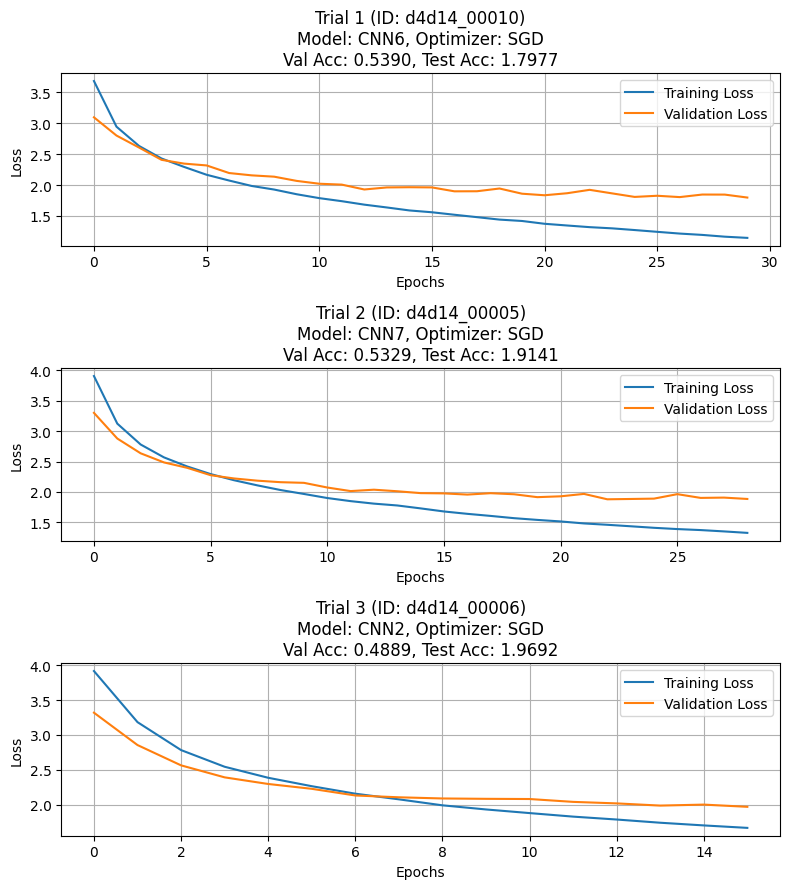
\includegraphics[width=1\linewidth]{training_plots.png}
    \caption{Model Selection Training/Validation Loss}
    \label{fig: model selection training/validation loss}
\end{figure}


\section{Best Model Architectures} \label{sec: best model architectures}
After evaluating the 60 models, the top \textbf{3 models} were selected based on their validation accuracy and were retrained on the entire training set (50,000 images).

% \subsubsection{Summary of components used within the 3 best models}

\subsubsection{Activation Functions} ReLU for models: CNN6, CNN2. And Leaky ReLU for CNN7.

\subsubsection{Optimizers} While experimenting, the following optimizers were included: Adam, RMSProp, AdaGrad, and SGD. However, while selecting the model with the ray tune, it only picked models with \textbf{SGD}.%, which was surprising. 

\subsubsection{Hyper-parameters for each model:}
\begin{itemize}
    \item \textbf{CNN6:}
          \begin{itemize}
              \item Optimizer: SGD
              \item Learning Rate: 0.004278%943210433503
              \item Momentum: 0.00958%1454091906229
              \item Dampening: 0.0946%55749224775
          \end{itemize}
    \item \textbf{CNN7:}
          \begin{itemize}
              \item Optimizer: SGD
              \item Learning Rate: 0.0390%65662473146474
              \item Momentum: 0.178957%6010660325
              \item Dampening: 0.34405%47236489297
          \end{itemize}
    \item \textbf{CNN2:}
          \begin{itemize}
              \item Optimizer: SGD
              \item Learning Rate: 0.0498%9411767043811
              \item Momentum: 0.0867%0108644990782
              \item Dampening: 0.0415%6399777574156
          \end{itemize}
\end{itemize}

Figure~\ref{fig:cnn_architectures} shows the three best model architectures. It shows the different convolution layers used with their perspective outputs, the activation functions, different normalization, and generalization layers and the fully connected layers.

\begin{figure}[H]
    % \vspace{-20pt}
    \small
    \centering
    % Define styles once to avoid repetition
    \tikzset{
        layer/.style = {rectangle, draw, rounded corners, align=center, minimum height=0.8cm, text width=4cm},
        arrow/.style = {->, thick},
        input/.style = {layer, fill=white!30},
        conv/.style = {layer, fill=red!40},
        fc/.style = {layer, fill=blue!20},
        bn_dropout/.style = {layer, fill=orange!40},
        activation/.style = {layer, fill=green!30},
        pooling/.style = {layer, fill=purple!40},
        flatten/.style = {layer, fill=white!10},
        legend_box/.style = {rectangle, draw, rounded corners, align=left, minimum height=0.5cm, text width=3cm, fill=white}
    }
    % Legend
    % \begin{subfigure}[b]{0.2\textwidth} 
    % \label{legend}
    % % \vspace{-10000pt}
    % \centering
    % \caption{Legend}
    % \begin{tikzpicture}[node distance=0.3cm, >=stealth, thick, scale=0.6, transform shape]
    %     % \node [legend_box] (legend1) { \textbf{Layer Types} };
    %     \node [conv] (legend_conv) {Conv2D};
    %     \node [fc, below=of legend_conv] (legend_fc) {Fully Connected};
    %     \node [bn_dropout, below=of legend_fc] (legend_bn_dropout) {BatchNorm/Dropout};
    %     \node [activation, below=of legend_bn_dropout] (legend_activation) {Activation Function};
    %     \node [pooling, below=of legend_activation] (legend_pooling) {Pooling Layer};
    %     \node [flatten, below=of legend_pooling] (legend_flatten) {Flatten Layer};
    %     \node [input, below=of legend_flatten] (legend_input) {Input Layer};
    % \end{tikzpicture}
    % \end{subfigure}
    % \hfill
    % CNN6 Subfigure
    \begin{subfigure}[b]{0.1\textwidth}
        \centering
        \caption{CNN6}
        \begin{tikzpicture}[node distance=0.5cm, >=stealth, thick, scale=0.6, transform shape]
            % Define nodes
            \node (input) [input] {Input Image \\ (3 channels) \\ Output: 32x32x3};
            \node (conv1) [conv, below=of input] {Conv2D: 3 $\rightarrow$ 128 \\ Kernel: 3x3, Padding: 1 \\ Output: 32x32x128};
            \node (bn1) [bn_dropout, below=of conv1] {BatchNorm \\ Output: 32x32x128};
            \node (relu1) [activation, below=of bn1] {ReLU Activation \\ Output: 32x32x128};
            \node (pool1) [pooling, below=of relu1] {Max Pooling \\ Kernel: 2x2, Stride: 2 \\ Output: 16x16x128};

            \node (conv2) [conv, below=of pool1] {Conv2D: 128 $\rightarrow$ 246 \\ Kernel: 3x3, Padding: 1 \\ Output: 16x16x246};
            \node (bn2) [bn_dropout, below=of conv2] {BatchNorm \\ Output: 16x16x246};
            \node (relu2) [activation, below=of bn2] {ReLU Activation \\ Output: 16x16x246};
            \node (pool2) [pooling, below=of relu2] {Max Pooling \\ Kernel: 2x2, Stride: 2 \\ Output: 8x8x246};

            \node (conv3) [conv, below=of pool2] {Conv2D: 246 $\rightarrow$ 256 \\ Kernel: 3x3, Padding: 1 \\ Output: 8x8x256};
            \node (bn3) [bn_dropout, below=of conv3] {BatchNorm \\ Output: 8x8x256};
            \node (relu3) [activation, below=of bn3] {ReLU Activation \\ Output: 8x8x256};

            % \node (flatten) [flatten, below=of relu3] {Flatten \\ Output: 16384};
            \node (fc1) [fc, below=of relu3] {Fully Connected \\ 16384 $\rightarrow$ 100 \\ (Output Layer) \\ Output: 100};

            % Draw arrows
            \draw [arrow] (input) -- (conv1);
            \draw [arrow] (conv1) -- (bn1);
            \draw [arrow] (bn1) -- (relu1);
            \draw [arrow] (relu1) -- (pool1);
            \draw [arrow] (pool1) -- (conv2);
            \draw [arrow] (conv2) -- (bn2);
            \draw [arrow] (bn2) -- (relu2);
            \draw [arrow] (relu2) -- (pool2);
            \draw [arrow] (pool2) -- (conv3);
            \draw [arrow] (conv3) -- (bn3);
            \draw [arrow] (bn3) -- (relu3);
            \draw [arrow] (relu3) -- (fc1);
            % \draw [arrow] (flatten) -- (fc1);
        \end{tikzpicture}
        \label{fig:CNN6}
    \end{subfigure}
    \hfill
    % CNN7 Subfigure
    \begin{subfigure}[b]{0.1\textwidth}
        \centering
        \caption{CNN7}
        \begin{tikzpicture}[node distance=0.3cm, >=stealth, thick, scale=0.6, transform shape]
            % Define nodes
            \node (input) [input] {Input Image \\ (3 channels) \\ Output: 32x32x3};
            \node (conv1) [conv, below=of input] {Conv2D: 3 $\rightarrow$ 38 \\ Kernel: 3x3, Padding: 1 \\ Output: 32x32x38};
            \node (bn1) [bn_dropout, below=of conv1] {BatchNorm \\ Output: 32x32x38};
            \node (leakyrelu1) [activation, below=of bn1] {Leaky ReLU \\ Output: 32x32x38};
            \node (pool1) [pooling, below=of leakyrelu1] {Max Pooling \\ Kernel: 2x2, Stride: 2 \\ Output: 16x16x38};
            \node (dropout1) [bn_dropout, below=of pool1] {Dropout \\ p=0.25 \\ Output: 16x16x38};

            \node (conv2) [conv, below=of dropout1] {Conv2D: 38 $\rightarrow$ 255 \\ Kernel: 3x3, Padding: 1 \\ Output: 16x16x255};
            \node (bn2) [bn_dropout, below=of conv2] {BatchNorm \\ Output: 16x16x255};
            \node (leakyrelu2) [activation, below=of bn2] {Leaky ReLU \\ Output: 16x16x255};
            \node (dropout2) [bn_dropout, below=of leakyrelu2] {Dropout \\ p=0.1 \\ Output: 16x16x255};

            \node (conv3) [conv, below=of dropout2] {Conv2D: 255 $\rightarrow$ 399 \\ Kernel: 3x3, Padding: 1 \\ Output: 16x16x399};
            \node (bn3) [bn_dropout, below=of conv3] {BatchNorm \\ Output: 16x16x399};
            \node (leakyrelu3) [activation, below=of bn3] {Leaky ReLU \\ Output: 16x16x399};
            \node (pool2) [pooling, below=of leakyrelu3] {Max Pooling \\ Kernel: 2x2, Stride: 2 \\ Output: 8x8x399};
            \node (dropout3) [bn_dropout, below=of pool2] {Dropout \\ p=0.1 \\ Output: 8x8x399};

            \node (conv4) [conv, below=of dropout3] {Conv2D: 399 $\rightarrow$ 200 \\ Kernel: 3x3, Padding: 1 \\ Output: 8x8x200};
            \node (bn4) [bn_dropout, below=of conv4] {BatchNorm \\ Output: 8x8x200};
            \node (leakyrelu4) [activation, below=of bn4] {Leaky ReLU \\ Output: 8x8x200};
            \node (dropout4) [bn_dropout, below=of leakyrelu4] {Dropout \\ p=0.1 \\ Output: 8x8x200};

            % \node (flatten) [flatten, below=of dropout4] {Flatten \\ Output: 12800};
            \node (fc1) [fc, below=of dropout4] {Fully Connected \\ 12800 $\rightarrow$ 100 \\ (Output Layer) \\ Output: 100};

            % Draw arrows
            \draw [arrow] (input) -- (conv1);
            \draw [arrow] (conv1) -- (bn1);
            \draw [arrow] (bn1) -- (leakyrelu1);
            \draw [arrow] (leakyrelu1) -- (pool1);
            \draw [arrow] (pool1) -- (dropout1);
            \draw [arrow] (dropout1) -- (conv2);
            \draw [arrow] (conv2) -- (bn2);
            \draw [arrow] (bn2) -- (leakyrelu2);
            \draw [arrow] (leakyrelu2) -- (dropout2);
            \draw [arrow] (dropout2) -- (conv3);
            \draw [arrow] (conv3) -- (bn3);
            \draw [arrow] (bn3) -- (leakyrelu3);
            \draw [arrow] (leakyrelu3) -- (pool2);
            \draw [arrow] (pool2) -- (dropout3);
            \draw [arrow] (dropout3) -- (conv4);
            \draw [arrow] (conv4) -- (bn4);
            \draw [arrow] (bn4) -- (leakyrelu4);
            \draw [arrow] (leakyrelu4) -- (dropout4);
            \draw [arrow] (dropout4) -- (fc1);
            % \draw [arrow] (flatten) -- (fc1);
        \end{tikzpicture}
        \label{fig:CNN7}
    \end{subfigure}
    \hfill
    % CNN2 Subfigure
    \begin{subfigure}[b]{0.1\textwidth}
        \centering
        \caption{CNN2}
        \begin{tikzpicture}[node distance=0.3cm, >=stealth, thick, scale=0.6, transform shape]
            % Define nodes
            \node (input) [input] {Input Image \\ (3 channels) \\ Output: 32x32x3};
            \node (conv1) [conv, below=of input] {Conv2D: 3 $\rightarrow$ 32 \\ Kernel: 3x3, Stride: 1, Padding: 1 \\ Output: 32x32x32};
            \node (bn1) [bn_dropout, below=of conv1] {BatchNorm \\ Output: 32x32x32};
            \node (relu1) [activation, below=of bn1] {ReLU \\ Output: 32x32x32};
            \node (conv2) [conv, below=of relu1] {Conv2D: 32 $\rightarrow$ 64 \\ Kernel: 3x3, Stride: 1, Padding: 1 \\ Output: 32x32x64};
            \node (bn2) [bn_dropout, below=of conv2] {BatchNorm \\ Output: 32x32x64};
            \node (relu2) [activation, below=of bn2] {ReLU \\ Output: 32x32x64};
            \node (pool1) [pooling, below=of relu2] {Max Pooling \\ Kernel: 2x2, Stride: 2 \\ Output: 16x16x64};

            \node (conv3) [conv, below=of pool1] {Conv2D: 64 $\rightarrow$ 150 \\ Kernel: 3x3, Stride: 1, Padding: 1 \\ Output: 16x16x150};
            \node (bn3) [bn_dropout, below=of conv3] {BatchNorm \\ Output: 16x16x150};
            \node (relu3) [activation, below=of bn3] {ReLU \\ Output: 16x16x150};
            \node (conv4) [conv, below=of relu3] {Conv2D: 150 $\rightarrow$ 300 \\ Kernel: 3x3, Stride: 1, Padding: 1 \\ Output: 16x16x300};
            \node (relu4) [activation, below=of conv4] {ReLU \\ Output: 16x16x300};
            \node (pool2) [pooling, below=of relu4] {Max Pooling \\ Kernel: 2x2, Stride: 2 \\ Output: 8x8x300};

            % \node (flatten) [flatten, below=of pool2] {Flatten \\ Output: 19200};
            \node (fc1) [fc, below=of pool2] {Fully Connected \\ 19200 $\rightarrow$ 512 \\ Output: 512};
            \node (relu5) [activation, below=of fc1] {ReLU \\ Output: 512};
            \node (dropout) [bn_dropout, below=of relu5] {Dropout \\ p=0.3 \\ Output: 512};
            \node (fc2) [fc, below=of dropout] {Fully Connected \\ 512 $\rightarrow$ 100 \\ (Output Layer) \\ Output: 100};

            % Draw arrows
            \draw [arrow] (input) -- (conv1);
            \draw [arrow] (conv1) -- (bn1);
            \draw [arrow] (bn1) -- (relu1);
            \draw [arrow] (relu1) -- (conv2);
            \draw [arrow] (conv2) -- (bn2);
            \draw [arrow] (bn2) -- (relu2);
            \draw [arrow] (relu2) -- (pool1);
            \draw [arrow] (pool1) -- (conv3);
            \draw [arrow] (conv3) -- (bn3);
            \draw [arrow] (bn3) -- (relu3);
            \draw [arrow] (relu3) -- (conv4);
            \draw [arrow] (conv4) -- (relu4);
            \draw [arrow] (relu4) -- (pool2);
            \draw [arrow] (pool2) -- (fc1);
            % \draw [arrow] (flatten) -- (fc1);
            \draw [arrow] (fc1) -- (relu5);
            \draw [arrow] (relu5) -- (dropout);
            \draw [arrow] (dropout) -- (fc2);
        \end{tikzpicture}
        \label{fig:CNN2}
    \end{subfigure}
    \hfill

    \caption{Architectures of CNN6, CNN7, and CNN2 }
    \label{fig:cnn_architectures}
\end{figure}




\subsubsection{Model Selection Graphs}

\section{Full retrain} \label{sec: full retrain}
After selecting the models, they were fully trained using the entire training set ( 50,000 ) images up to 100 epochs.
Figure ~\ref{fig: full data training} shows the training loss of the 3 best models. Note that there is no validation loss because, at this point, all the training data was used for training.
\begin{figure}[H]
    \centering
    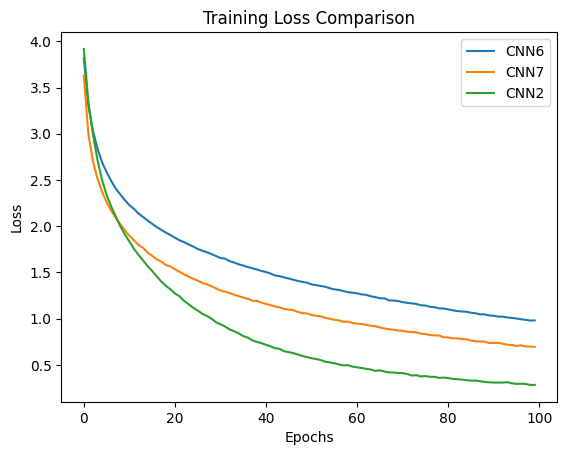
\includegraphics[width=1\linewidth]{Full_Data_Training.png}
    \caption{Full Data Training}
    \label{fig: full data training}
\end{figure}

\subsection{Test Accuracies }
\begin{itemize}
    \item CNN6: 60.1\%
    \item CNN7: 61.1\%
    \item CNN2: 58.7\%
\end{itemize}




\section{Comparison with top Models} \label{sec: comparision}
To compare these 3 best models, I used projects from \href{https://paperswithcode.com/sota/image-classification-on-cifar-100 }{papers with code} that focus on training a model only on CIFAR100.
The top 4 models found are
\begin{itemize}
    \item \textbf{\href{https://paperswithcode.com/paper/exact-how-to-train-your-accuracy}{EXACT: How to Train Your Accuracy}} - with an accuracy of 82.68
    \item \textbf{\href{https://paperswithcode.com/paper/differentiable-spike-rethinking-gradient}{Differentiable Spike: Rethinking Gradient-Descent for Training Spiking Neural Networks}} - with an accuracy of 74.24
    \item \textbf{\href{https://paperswithcode.com/paper/beta-rank-a-robust-convolutional-filter}{Beta-Rank: A Robust Convolutional Filter Pruning Method For Imbalanced Medical Image Analysis}} - with an accuracy of 74.01
    \item \textbf{\href{https://paperswithcode.com/paper/deep-residual-networks-with-exponential}{Deep Residual Networks with Exponential Linear Unit}} with an accuracy of 73.5
\end{itemize}

Taking an average of all three would give an average accuracy of 76.11\%, and comparing it with the models developed here.
The top models from papers with code perform about 16\% better, which is comparable since I only focus on training this model for 1-2 weeks. The author of these competitive projects used more time to experiment and develop new ideas to improve their performance. Models that performed with 60\% accuracy are ranked in the \~180 positions, and with 50\% accuracy are ranked in the 192 positions.


\section{Total number of parameters}
\begin{itemize}
    \item CNN6 Total Parameters: 2,494,022
    \item CNN7 Total Parameters: 3,004,917
    \item CNN2 Total Parameters: 10,393,946
\end{itemize}

% TO calcualte the number of parameters 
% I traversed through the layers using  \verb|net.named_parameters()| and got the number of parameters using the \verb|numel()| method. 

% \subsection*{Model: CNN6}
% % \noindent\textbf{Layer-wise parameters:}
% To calculate the parameters, we can multiply all the input sizes of the conv layers and add the bias; batch norm contains 2 per feature. The pooling layers do not contain any parameters. 
% Below are the calculations for CNN6, which aligns with what  t
% \begin{enumerate}
%     \item \textbf{Layer 1}
%     \begin{itemize}
%         \item Conv2d (Input: 3, Output: 128): $3 \times 128 \times 3 \times 3 = 3,456$ parameters
%         \item Bias: $128$ parameters
%         \item BatchNorm2d (128 features): $128 \times 2 = 256$ parameters
%         \item \textbf{Total Layer 1:} $3,456 + 128 + 256 = 3,840$ parameters
%     \end{itemize}
%     \item \textbf{Layer 2}
%     \begin{itemize}
%         \item Conv2d (128 $\rightarrow$ 246): $128 \times 246 \times 3 \times 3 = 283,392$ parameters
%         \item Bias: $246$ parameters
%         \item BatchNorm2d (246 features): $246 \times 2 = 492$ parameters
%         \item \textbf{Total Layer 2:} $283,392 + 246 + 492 = 284,130$ parameters
%     \end{itemize}
%     \item \textbf{Layer 3}
%     \begin{itemize}
%         \item Conv2d (246 $\rightarrow$ 256): $246 \times 256 \times 3 \times 3 = 566,784$ parameters
%         \item Bias: $256$ parameters
%         \item BatchNorm2d (256 features): $256 \times 2 = 512$ parameters
%         \item \textbf{Total Layer 3:} $566,784 + 256 + 512 = 567,552$ parameters
%     \end{itemize}
%     \item \textbf{Fully Connected Layer}
%     \begin{itemize}
%         \item Linear (16,384 $\rightarrow$ 100): $16,384 \times 100 = 1,638,400$ parameters
%         \item Bias: $100$ parameters
%         \item \textbf{Total FC Layer:} $1,638,400 + 100 = 1,638,500$ parameters
%     \end{itemize}
% \end{enumerate}

% \subsection*{Model: CNN7}

% \begin{itemize}
%     \item \textbf{Total parameters:} 3,004,917
%     \item \textbf{Trainable parameters:} 3,004,917
% \end{itemize}

% \noindent\textbf{Layer-wise parameters:}

% \begin{enumerate}
%     \item \textbf{Layer 1}
%     \begin{itemize}
%         \item Conv2d (3 $\rightarrow$ 38): $3 \times 38 \times 3 \times 3 = 1,026$ parameters
%         \item Bias: $38$ parameters
%         \item BatchNorm2d (38 features): $38 \times 2 = 76$ parameters
%         \item \textbf{Total Layer 1:} $1,026 + 38 + 76 = 1,140$ parameters
%     \end{itemize}
%     \item \textbf{Layer 2}
%     \begin{itemize}
%         \item Conv2d (38 $\rightarrow$ 255): $38 \times 255 \times 3 \times 3 = 261,270$ parameters
%         \item Bias: $255$ parameters
%         \item BatchNorm2d (255 features): $255 \times 2 = 510$ parameters
%         \item \textbf{Total Layer 2:} $261,270 + 255 + 510 = 262,035$ parameters
%     \end{itemize}
%     \item \textbf{Layer 3}
%     \begin{itemize}
%         \item Conv2d (255 $\rightarrow$ 399): $255 \times 399 \times 3 \times 3 = 916,725$ parameters
%         \item Bias: $399$ parameters
%         \item BatchNorm2d (399 features): $399 \times 2 = 798$ parameters
%         \item \textbf{Total Layer 3:} $916,725 + 399 + 798 = 917,922$ parameters
%     \end{itemize}
%     \item \textbf{Layer 4}
%     \begin{itemize}
%         \item Conv2d (399 $\rightarrow$ 200): $399 \times 200 \times 3 \times 3 = 718,200$ parameters
%         \item Bias: $200$ parameters
%         \item BatchNorm2d (200 features): $200 \times 2 = 400$ parameters
%         \item \textbf{Total Layer 4:} $718,200 + 200 + 400 = 718,800$ parameters
%     \end{itemize}
%     \item \textbf{Fully Connected Layer}
%     \begin{itemize}
%         \item Linear (12,800 $\rightarrow$ 100): $12,800 \times 100 = 1,280,000$ parameters
%         \item Bias: $100$ parameters
%         \item \textbf{Total FC Layer:} $1,280,000 + 100 = 1,280,100$ parameters
%     \end{itemize}
% \end{enumerate}

% \subsection*{Model: CNN2}

% \begin{itemize}
%     \item \textbf{Total parameters:} 10,393,946
%     \item \textbf{Trainable parameters:} 10,393,946
% \end{itemize}

% \noindent\textbf{Layer-wise parameters:}

% \begin{enumerate}
%     \item \textbf{Layer 1}
%     \begin{itemize}
%         \item Conv2d (3 $\rightarrow$ 32): $3 \times 32 \times 3 \times 3 = 864$ parameters
%         \item Bias: $32$ parameters
%         \item BatchNorm2d (32 features): $32 \times 2 = 64$ parameters
%         \item Conv2d (32 $\rightarrow$ 64): $32 \times 64 \times 3 \times 3 = 18,432$ parameters
%         \item Bias: $64$ parameters
%         \item BatchNorm2d (64 features): $64 \times 2 = 128$ parameters
%         \item \textbf{Total Layer 1:} $864 + 32 + 64 + 18,432 + 64 + 128 = 19,584$ parameters
%     \end{itemize}
%     \item \textbf{Layer 2}
%     \begin{itemize}
%         \item Conv2d (64 $\rightarrow$ 150): $64 \times 150 \times 3 \times 3 = 86,400$ parameters
%         \item Bias: $150$ parameters
%         \item BatchNorm2d (150 features): $150 \times 2 = 300$ parameters
%         \item Conv2d (150 $\rightarrow$ 300): $150 \times 300 \times 3 \times 3 = 405,000$ parameters
%         \item Bias: $300$ parameters
%         \item \textbf{Total Layer 2:} $86,400 + 150 + 300 + 405,000 + 300 = 492,150$ parameters
%     \end{itemize}
%     \item \textbf{Fully Connected Layers}
%     \begin{itemize}
%         \item Linear (19,200 $\rightarrow$ 512): $19,200 \times 512 = 9,830,400$ parameters
%         \item Bias: $512$ parameters
%         \item Linear (512 $\rightarrow$ 100): $512 \times 100 = 51,200$ parameters
%         \item Bias: $100$ parameters
%         \item \textbf{Total FC Layers:} $9,830,400 + 512 + 51,200 + 100 = 9,882,212$ parameters
%     \end{itemize}
% \end{enumerate}
\section{Conclusion} \label{sec: conclusion}
The three CNN models developed performed well when trained solely on CIFAR100 data aided by data transformations, generalization and normalization layers, and ray tune for model selection.
%However, they are expected not to perform exceptionally because the number of classes is high and the number of sample data per class is low. 


% The three CNN models described above were selected after training 50 models with Ray Tune for hyper-parameter optimization. The data was carefully split into training and validation sets, and data augmentation techniques were employed to enhance model generalization. CNN2 emerged as the best-performing model, achieving the highest test accuracy with fewer parameters compared to CNN6 and CNN7. Further experimentation with different optimizers and regularization techniques could potentially improve the models even more.

\end{document}